\chapter{State of the art}
\label{ch:sota}

\section{Churn prediction}

We organize our presentation of the state of the art in churn prediction by
considering 4 aspects of interest in a usual churn prediction process: learning
algorithm, data preprocessing, class balancing and choice of an evaluation
measure.

\subsection{Learning algorithm}

A large number of machine learning models have been applied to churn prediction
in the literature. While some studies focus on simple and interpretable models
such as decision tree \parencite{keramati2014improved} or logistic regression
\parencite{olle2014hybrid}, other studies prefer the use of more complex models,
at the expense of direct interpretation. These methods include boosting applied
on simple classifiers \parencite{vafeiadis2015comparison}, random forests,
support vector machine, neural networks, among others
\parencite{umayaparvathi2016attribute, verbeke2012new}. An extensive overview of
the current trends in churn prediction modeling is given in
\parencite{kayaalp2017review}. We describe in this section the learning
algorithms used most often according to this review.

A decision tree is a non-linear model that partitions the input space into
mutually exclusive regions, and each of these regions is assigned a mapping
between the input vector and the output value. In the case of a classification
tree, each region is assigned a label. The partition of the input space is
determined by a tree structure composed of internal nodes and terminal nodes.
Each internal node is associated with a rule that determines which child node
should be visited next, based on the value of one of the variables. Each of the
terminal nodes is associated with a mapping function,  a label in the case of a
classification tree. The main methods of decision tree inductions are ID3
\parencite{quinlan1986induction}, C4 \parencite{quinlan1987simplifying}, and
CART \parencite{breiman1984classification}.

Logistic regression is a statistical binary classification model that assigns a
probability to each point of the input space. The probability of an input vector
$\bm x = [x_1,\dots,x_n]$ is calculated as the application of the sigmoid function on a linear
combination of the values in $\bm x$. More precisely, to each variable $X_i$ is
assigned a coefficient $w_i$, and an intercept coefficient $w_0$ is also
defined. The predicted probability of a logistic regression model is thus

\begin{equation*}
    s(\bm x) = \frac{1}{1+\exp{(-(w_0 + w_1x_1 + \dots + w_nx_n))}}.
\end{equation*}

The weights $w_0,\dots,w_n$ can be learned by maximizing their log-likelihood
given a set of learning examples using the gradient descent algorithm.

Artificial neural networks are computational models that process input in a
distributed, parallel fashion. They are initially inspired by biological
neurons, but their current development has moved towards a more rigorous
interpretation based on theoretical machine learning. A wide variety of neural
network architectures exists, but we present here only \emph{feed-forward neural
networks} (FNN) for their prominent use in the churn prediction literature. A
MLP consists of a series of layers, and each layer comprises multiple neurons.
In the fully connected configuration, a neuron takes as input all outputs from
the previous layer. The output of the neuron is the result of applying a
non-linear activation function to the dot product of the inputs with a vector of
weights. Many  activation functions exist, such as the sigmoid function, the
rectified linear unit \parencite{nair2010rectified}, the hyperbolic tangent, and
many others \parencite{cheng1994neural}. The weights of each inter-neuron link
are learned by gradient descent on a loss function given training samples. The
exact learning setup can vary widely, thanks to the numerous possibilities in
the choice of the loss function and the gradient descent implementation.

A support vector machine (SVM) is a geometrical classification model based on
the notion of \emph{maximum margin hyperplane}. A SVM model splits the input
space into two separate regions by using a hyperplane. This hyperplane is chosen
as to maximize its distance to the nearest data point in either class. In
order to handle arbitrary input space or non-separable classes, a kernel
function is used to project the input space into a well-known Hilbert space.
Also, slack variables can be introduced to relax the strict requirement that the
margin should perfectly separate the two classes. The geometrical formulation of
this model enables an exact optimization procedure based on the dual of the
Lagrangian. One of the first modern formulations of the SVM model is given in
\parencite{boser1992training}.

A random forest is an ensemble model composed of multiple decision trees. One of
the first descriptions of this model is given in \textcite{breiman2001random}.
Each tree is constructed from a subset of samples and using only a subset of the
variables. In the case of a classification task, each of the individual trees
votes for the output label of a given data example, whereas in the case of a
regression task, the output is the average prediction of all trees. The
intuition is to obtain a set of deep trees having a high variance but low biais.
The average of these trees has thus a lower variance than each individual tree,
as long as these trees are uncorrelated. The tree are made uncorrelated by
sampling independently the set of samples and variables used to train each of
them.

\subsection{Data preprocessing}

While the choice of model is important, it is equally important to consider a
proper choice of features, data preprocessing and evaluation measure. Feature
choice is limited by the available data infrastructure and usually consists of
call detail records on the course of a few weeks. \textcite{huang2012customer}
presented however how new kinds of features, including demographics profiles,
marketing segments, and complaint information, can improve prediction accuracy.

Data preprocessing refers to the process following data acquisition and
consists of modifying the data in various ways before the use in a predictive
model. This comprises, non-exhaustively, feature engineering, data reduction,
anomalies removal, encoding of categorical variables, and data normalization
\parencite{zhang2003data}. \textcite{coussement2017comparative} give an overview
of common preprocessing steps used in churn prediction, and how careful
preprocessing can positively affect the performance of the model. They even show
that a simple logistic regression model applied to optimally preprocessed data
competes with complex learning algorithms such as neural network or support
vector machine applied on data preprocessed with a basic preparation procedure.

Recent years have witnessed the widespread usage of network-based classification
for churn prediction. \textcite{verbeke2014social} present some experiment in
this area of research. \parencite{oskarsdottir2017social} perform an extensive
benchmark of the different techniques proposed in the literature. The approach
is based on call detail records (CDR) containing the communication logs of the
subscribers. This data can be organized as a graph where nodes represent
customers and edges represent social ties between customers. The basic
assumption of network-based classifiers, which use such graphs to classify
customers as churners or non-churners, is that customers having social ties with
churners are more likely to churn themselves. This assumption is purposely
loosely defined, as its exact implementation implies different assumptions and
modeling decisions \parencite{oskarsdottir2017social}. From that, one can either
construct a predictive model that directly uses the social graph, or extract
features from the network and use them as the input of a conventional
classifier, or even combine the two approaches. The outcome of the two articles
is that relational and classical non-relational classifiers detect different
types of churners and that a combination of both types of classifiers
approaches performs best.

\textcite{oskarsdottir2018time} present a novel, end-to-end approach to the
problem of churn detection where a time-varying social network of the customer
base is constructed, and a multivariate time series is then extracted for each
customer from this network. Then, different time series classifiers are used to
predict churn. A novel multivariate time series classifier is proposed, an
adaptation of the similarity forest classifier \parencite{sathe2017similarity}.
\textcite{oskarsdottir2018time} conclude that their approach outperforms
state-of-the-art time series classifiers and non-time-based models for early
churn prediction. However, static random forest and logistic regression are
better at predicting late churn (that is, on short time scales).

\subsection{Class balancing}
\label{sec:sota_balancing}

It is important to consider class imbalance when designing models for churn
prediction. Indeed, the number of churners is usually very low compared to the
total number of customers, and most machine learning models are usually not
suited to handle highly imbalanced data \parencite{batista2004study}. Class
balancing techniques have to be used to tackle this problem. These techniques
can roughly be divided into three categories: data-level balancing, model-level
balancing, and ensemble methods.

Data-level balancing consists in modifying the dataset by either decreasing the
number of majority instances, increasing the number of minority instances, or
both. Random oversampling (ROS) consists in randomly replicating instances of
the minority class, whereas random undersampling (RUS) randomly eliminates
instances of the majority class. ROS increases the risk of overfitting, by
replicating exactly existing examples, whereas RUS loses information by removing
potentially useful examples, thus increasing variance. Synthetic minority
oversampling technique (SMOTE) \parencite{chawla2002smote} addresses the
overfitting issue by creating new instances of the minority class with linear
interpolations between minority example and their nearest neighbors. Several
variations and improvements exist, such as ADASYN \parencite{he2008adasyn} and
MWMOTE \parencite{barua2014mwmote}. Intelligent undersampling techniques also
exist, such as the one-sided selection (OSS) \parencite{kubat1997addressing}
that removes redundant or borderline majority instances, or the cluster-based
undersampling (CLUS) \parencite{yen2009cluster} that groups majority instances
into clusters, and reduce the number of instances in each cluster.
\textcite{dal2015undersampling} provide a condition under which undersampling
improves the ranking of test instances, which depends on the class balance rate,
the nonseparability of the data, and the variance of the learning algorithm.
This highlights the fact that no unique undersampling strategy is adapted to all
problems.

Model-level balancing consists in modifying the learning algorithm in such a way
that minority instances are given more importance, often through the use of
asymmetric misclassification costs. \textcite{ting2002instance} applied this
methodology to classification trees, and \textcite{veropoulos1999controlling} to
support vector machines.

Ensemble methods for class imbalance combine multiple models to obtain a better
overall model while taking into account class imbalance. For example, Roughly
Balanced Bagging \parencite{hido2009roughly} uses bagging to create multiple
classifiers, each being trained by undersampling using a number of majority
instances determined by a negative binomial distribution.
\textcite{chen2004using} proposes integrating balancing by random undersampling
or misclassification weighting into the random forest algorithm.

Since we use the ensemble balancing method \emph{EasyEnsemble}
\parencite{liu2009exploratory} in this thesis, we present it here in more
details. Given the set of positive instances $\mathcal P$ and the set of
negative instances $\mathcal N$, data-level undersampling methods consist in
choosing a subset $\mathcal N'\subset \mathcal N$ such that, by training on
$|\mathcal N'|\cup|\mathcal P|$, the ratio between positive and negative
instances is suitable for a given learning algorithm. It is common to choose a
ratio of 1. The main issue with this approach is that a large number of positive
instances (i.e. all of $\mathcal N \setminus \mathcal N'$) is ignored, thus
increasing the variance of the resulting trained model. EasyEnsemble overcomes
this issue by independently sampling $T>1$ subsets $\mathcal N_1,\dots,\mathcal
N_T$ from $\mathcal N$. Then, $T$ predictive models are trained on all of
$\mathcal P$ and individually on each $\mathcal N_i$. The final predictions are
the average of the predictions of the $T$ models. This process is pictured in
figure \ref{fig:easy_ensemble_diagram}. In our case, the predictive models are
random forests.

\begin{figure}
    \centering
	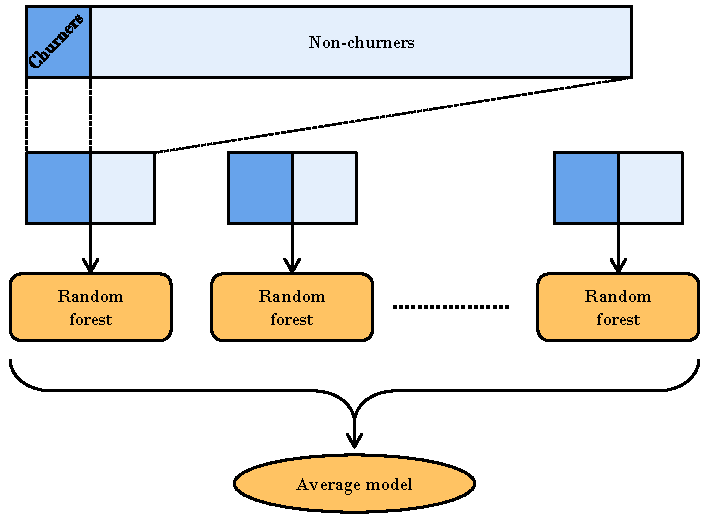
\includegraphics[width=0.9\linewidth]{figures/easy_ensemble_diagram.pdf}
	\caption{Easy ensemble methodology for unbalanced data. A set of random
	forests is trained each on the whole set of positive instances, and on a
	randomly chosen subset of negative instances. The final predictions are
	the average of all the random forests individual predictions.}
	\label{fig:easy_ensemble_diagram}
\end{figure}

\textcite{dal2013racing} showed that no unique class balancing method works best
in all situations, and the they should be evaluated and selected on a case by
case basis. An extensive overview and comparison of class balancing techniques
in churn prediction is given in \parencite{zhu2017empirical}.
\textcite{dal2014learned} compared several balancing techniques in the context
of credit card fraud detection, as well as solutions for other aspects of the
fraud detection problem (online learning and concept drift).

\subsection{Evaluation measure}

The last step of a predictive model assessment is the evaluation of
classification performance. Several performance measures exist for this purpose,
such as precision, recall, F-score, area under the receiver operating
characteristic curve (AUC), lift, maximum profit criterion, and expected maximum
profit criterion. We briefly explain here these measures and their current use
in the literature.

We first introduce the notion of confusion matrix, as shown in table
\ref{tab:confusion_mat}. The fact that a customer is a churner or not is labeled
by the value of $y$, and corresponds the first column. We also write a churner
as an ``actual P'' (for \emph{positive} instance), and similarly a non-churner
as ``actual N'' (for \emph{negative} instance). The prediction of a
classification algorithm for a customer is a score $s$. If this score is larger
than a chosen threshold $t$, then the customer is predicted to be a churner,
written ``predicted P''. Similarly, if the score $s$ is below the threshold $t$,
the customer is predicted not to be a churner, written ``predicted N''. The
four possible combinations that these two conditions yield are presented
in the confusion matrix in table \ref{tab:confusion_mat}. The value of each
cell (TP, FP, FN, and TN) denotes the number of instances which meet both of the
corresponding criteria.

\begin{table}
    \centering
    \begin{tabular}{r|cc}
        & Predicted P ($s>t$) & Predicted N ($s\le t$) \\[15pt]
        \hline
        & & \\
        Actual P ($y=1$) & True positives ($\TP\,$) & False negatives ($\FN\,$) \\[15pt]

        & & \\
        Actual N ($y=0$) & False positives ($\FP\,$) & True negatives ($\TN\,$) \\[15pt]
    \end{tabular}
    \caption{Confusion matrix.}
    \label{tab:confusion_mat}
\end{table}

Precision is the fraction of true churners among all those we predicted to be
churners, and recall is the fraction of predicted churners among all the true
churners in the population.

\begin{equation*}
    \precision = P(y=1|S>t) = \frac{\TP}{\TP + \FP}
\end{equation*}
\begin{equation*}
    \recall    = P(S>t|y=1) = \frac{\TP}{\TP + \FN}
\end{equation*}

In order to optimize both of these scores at the same time, one can use the
F-score (also called F1 score, or F-measure), which is the harmonic mean of
precision and recall.

\[\Fmeasure = \frac{2\times \precision \times \recall}{\precision + \recall}\]

By using the harmonic mean, we punish low values in any of the two values. It is
sometimes used in the churn prediction literature \parencite{ahmed2017churn,
keramati2014improved}.

Receiver operating characteristic (ROC) curve \parencite{krzanowski2009roc} is a
plot of all possible compromises between true positive rate (TPR) and false
positive rate (FPR). TPR is another name for recall, and FPR is the fraction of
non-churners falsely predicted to be churners, among all non-churners.

\begin{equation*}
    \FPR=P(S>t|y=0)=\frac{\FP}{\FP + \TN}
\end{equation*}

In order to compare the ROC curve of different models, we use the area under the
curve (AUC) as a measure of performance.

\[\AUC=\int_{-\infty}^{+\infty}F_1(s)f_0(s)ds\]

AUC is very often used in churn prediction \parencite{coussement2017comparative,
mitrovic2018operational} because it is less sensitive to class imbalance (few
churners in a large population of customers) and misclassification cost
\parencite{verbeke2012new}.

An important drawback of these performance measures is that they do not
represent the real objective of churn prediction: given that we are
certainly not able to offer an incentive to all customers likely to
churn, we have to restrict the retention campaign to a limited number of
customers. From that, we wish to minimize the number of misclassifications
occurring in this small subset of customers. This is the definition of the lift:
given a certain set of customers (usually the subset of the customers with the
highest predicted probability of churn), the lift is the ratio between the churn
rate in this set and the churn rate in the whole customer base.

\[\lift(t) = \frac{P(y=1|S>t)}{P(y=1)}\]

The value of the lift indicates how much we do better than choosing customers at
random. For example, a lift of 3 indicates that the model will give a set of
customers with 3 times as much churners as if we picked that many customers at
random. The number of customers to consider is dependent on the application (it
should ideally be the number of customers reachable by the retention campaign),
but a lift at 10\% is sometimes used as a baseline \parencite{zhu2017empirical,
verbeke2014social}.

In order to determine formally how many customers should be included in the
retention campaign, and therefore in the lift measure, \textcite{verbeke2012new}
developed the maximum profit criterion (MPC) and the expected maximum profit
criterion (EMPC) \parencite{verbeke2012new, verbraken2013novel}. These two
measures consist of evaluating the expected costs and benefits of conducting a
retention campaign and selecting the optimal number of customers to call. The
difference between MPC and EMPC is that MPC considers the cost and benefits to
be known and fixed, while EMPC assigns a probability density function to these
parameters. MPC and EMPC are often used in churn prediction
\parencite{zhu2017empirical, oskarsdottir2018time, stripling2018profit}.

\section{Causal analysis}
\label{sec:sota_caus}

Finding and using causes is crucial in human reasoning and decision making.
While a predictive model returns the probability of a target value given that we
observe a certain input vector, a causal model is supposed to return the target
probability given that we set (e.g. by intervention) that input. The aim of
causal analysis is to determine the consequences of manipulations and is opposed
to the process of making predictions from observations. When used as a feature
selection criterion, it enables increased robustness to violation of the
assumption of independent and identical distributions (e.g. concept drift)
\parencite{guyon2007causal} and an enhanced understanding of the mechanism
underlying the data. The gold standard for causal modeling is to carry out
\emph{randomized controlled experiments} \parencite{fisher1937design}. For
example, in order to assess the influence of moderate wine consumption on heart
disease, it is not enough to measure wine consumption and heart disease in the
population. This may lead to erroneous conclusions, such as a socio-economic
factor that causes both increased wine consumption and risks of heart disease.
In order to avoid such a problem, one may assign to a randomly chosen group of
people a moderate wine consumption. If this group then shows a significantly
different risk of heart disease, then we may conclude that a causal relationship
indeed exists, and the apparent correlation is not due to a confounding factor.
However, such experiments may be expensive, unethical, difficult to implement or
unfeasible. This, along with advances in computation, data storage capabilities
and new machine learning techniques, led to the development of causal inference
based on observational data. We review here 5 approaches to data-driven causal
inference:

\begin{itemize}
    \item Bayesian network learning
    \item Markov blanket inference
    \item Information-theoretic filters
    \item Bivariate methods
    \item Supervised methods
\end{itemize}

All the approaches model causal relationships between random variables. These
random variables represent, for example, the different features available about
a customer in the churn prevention problem.

\subsection{Bayesian network learning}

A causal Bayesian network is a discrete acyclic graph where the set of nodes
correspond to the set of random variables, and a directed link indicates a
causal relationship between two variables. This graph is also accompanied by the
joint probability distribution of the set of random variables. Two conditions
are usually imposed on the graph and the probability distribution (the causal
Markov condition and the causal faithfulness condition, explained in section
\ref{sec:causal_intro}) to ensure that it respects the semantics of a causal
model. Notably, these conditions also allow predicting the effect of a
manipulation \parencite{spirtes2010introduction}. Causal Bayesian network can be
learned from observational data, and two types of procedures have been developed
for that purpose. The first one consists in a search in the graph structure
space, and optimization a fitness function. This approach is detailed in
\parencite{heckerman1998tutorial}. The second one is based on independence tests
between pairs of variables, and iteratively construct and orient edges until a
valid class of causal graphs is found. The PC and FCI algorithms use this
approach \parencite{spirtes1993causation}.

\subsection{Markov blanket inference}

The Markov blanket of a given target variable in a Bayesian network is a minimal
set of variables that are shielding the target variable from the influence of
other variables in the network. A formal definition is given in section
\ref{sec:causal_intro}. This subset of variables contains all the information
needed to predict the target variable (that is, any additional variable would be
redundant). Moreover, if the causal Markov and faithfulness assumptions hold,
then this Markov blanket is the set of direct causes (parents), direct effect
(children), and also the direct causes of the direct effects (spouses).
Inferring the Markov blanket of a variable, as opposed to inferring the complete
Bayesian network, is beneficial when the number of variables is large, such as
in microarray data. Several algorithms exist for Markov blanket inference,
notably KS \parencite{koller1996towards}, GS \parencite{margaritis2000bayesian}
IAMB \parencite{tsamardinos2003time}, HITON \parencite{aliferis2003hiton}, and
MMPB \parencite{tsamardinos2003time}. These algorithms start with an empty
Markov blanket and search for parents, children, and spouses of the target
variable by using conditional independence tests. A number of heuristics are
used to speed up the search, and most of these algorithms also include a second
phase where false positives are removed from the result.

\subsection{Information-theoretic filters}

A filter algorithm is a feature selection method that provides a ranking of the
input variables, based on some measure of statistical association with the
target variable. The best ranked variables are then selected in order to reduce
the computational requirements of the learning algorithm. Usual filter variable
selection methods suffer from several drawbacks. For example, multiple variables
may all provide the same information about the target (the extreme case
occurring when a variable is actually a copy of another). In a univariate
ranking approach, all of these variables would be included in the result, even
though one is sufficient. Another typical problem occurs when two or more
variables are not very predictive when taken individually, but on the contrary,
are predictive once used conjointly. These notions can be formalized using
information theory, and information-theoretic filters are designed to avoid the
exposed pitfalls. Another advantage of such filters is that they do not make any
assumption about the statistical distribution on the variables, thanks to the
use of mutual information as a dependency measure. State-of-the-art
information-theoretic filters include mRMR \parencite{peng2005feature}, DISR
\parencite{meyer2008information}, REL \parencite{bell2000formalism}, CMIM
\parencite{fleuret2004fast} and FCBF \parencite{yu2004efficient}. These
algorithms vary on whether or not they take complementarity into account, if
they avoid the estimation of multivariate density and if they return a ranking
of the variable (as opposed to an unordered set of relevant variables). These
filters can also be designed to explicitly favor variables having a direct
causal influence on the target, thanks to dependence relationships uniquely
exhibited by children, spouses and parents of the target. This is the case of
the mIMR \parencite{bontempi2010causal} and the MIMO
\parencite{bontempi2011multiple} filters.

\subsection{Bivariate methods}

In the last decade, there is an increased interest in telling cause from effect
from observational data on just two variables. This task is based on asymmetric
properties of the joint distribution of the two variables, and because of the
limited number of possible causal configurations, usual classification metrics
can be used to assess the performance of inference methods. Moreover, the nature
of the problem allows using classical machine learning algorithms for
cause/effect classification. This approach gained interest through the
organization of public a public challenge on Kaggle
(\url{https://www.kaggle.com/c/cause-effect-pairs}). This competition resulted
in several novel solutions for cause-effect detection, and a general advance in
the state of the art. The winner of the challenge, the team \emph{ProtoML},
extracts a large number of features from the variable distributions and uses a
large number of models for classification. The second-ranked participant,
\emph{jarfo} \cite{fonollosa2016conditional}, uses conditional distributions and
other information-theoretic quantities to infer features that are used for
prediction. The general outcome of this challenge is that asymmetries in causal
patterns enable the development of bivariate causal distinguishers, with an
accuracy significantly better than random.

\subsection{Supervised methods}

In the context of the aforementioned cause-effect pair competition,
\textcite{bontempi2015dependency} proposed an algorithm using asymmetries in the
conditional distributions of the variables. They extended their method to a
setting with more than two variables, by also extracting distribution features
from other variables and using them to infer the existence and direction of a
causal link in the two initial variables. This benefit is striking in the case
of a collider configuration $x_1 \rightarrow x_2 \leftarrow x_3$: in this case,
the dependency (or independence) between $x_1$ and $x_3$ tells us more about the
link $x_1 \rightarrow x_2$ than the dependency between $x_1$ and $x_2$. By using
a learning machine such as random forest, these features can be used to
successfully infer causal links, competing with and often outperforming
state-of-the-art Bayesian network inference methods.
